\documentclass[conference]{IEEEtran}
\IEEEoverridecommandlockouts
\usepackage{cite}
\usepackage{amsmath,amssymb,amsfonts}
\usepackage{algorithmic}
\usepackage{graphicx}
\usepackage{textcomp}
\usepackage{xcolor}
\usepackage{makecell}
\usepackage{hyperref}
\def\BibTeX{{\rm B\kern-.05em{\sc i\kern-.025em b}\kern-.08em
    T\kern-.1667em\lower.7ex\hbox{E}\kern-.125emX}}
\begin{document}

\title{Anti-Distillation: Knowledge Transfer from a Simple Model to the Complex One}

\author{\IEEEauthorblockN{Kseniia Petrushina}
\IEEEauthorblockA{\textit{Moscow Institute of Physics and Technology} \\
Moscow, Russia \\
petrushina.ke@phystech.edu}
\and
\IEEEauthorblockN{Oleg Bakhteev}
\IEEEauthorblockA{\textit{Moscow Institute of Physics and Technology} \\
\textit{FRC CSC of the RAS}\\
Moscow, Russia \\
bakhteev@phystech.edu}
\and
\IEEEauthorblockN{Andrey Grabovoy}
\IEEEauthorblockA{\textit{Moscow Institute of Physics and Technology} \\
\textit{Antiplagiat Company}\\
Moscow, Russia \\
grabovoy.av@phystech.edu}
\and
\IEEEauthorblockN{Vadim Strijov}
\IEEEauthorblockA{
\textit{FRC CSC of the RAS}\\
Moscow, Russia \\
strijov@phystech.edu}
}

\maketitle

\begin{abstract}
	The paper considers the problem of adapting the model to new data with a large amount of information. We propose to build a more complex model using the parameters of a simple one. We take into account not only the accuracy of the prediction on the original samples but also the adaptability to new data and the robustness of the obtained solution. The work is devoted to developing the method that allows adapting the pre-trained model to a more heterogeneous dataset. In the computational experiment, we analyse the quality of predictions and model robustness on Fashion-MNIST dataset.
\end{abstract}

\begin{IEEEkeywords}
knowledge transfer, weight initialization, distillation
\end{IEEEkeywords}

\section{Introduction}

Training a model from scratch, especially large neural net, usually take a long time. To get better results faster, researchers have been developing various methods allowing to use existing trained models to solve new problems. For instance, there are knowledge distillation~\cite{hinton2015distilling, lopezpaz2016unifying}, transfer learning~\cite{zhuang2019acomprehensive}, fine-tuning, low-rank model approximation~\cite{yu2017oncompressing}. Moreover, there are methods for initializing model parameters for faster convergence~\cite{glorot2010understanding, Koturwar2017WeightIO}. These approaches help to decrease the time needed for training or inference and achieve high quality~\cite{pmlr-v157-skorski21a}.

The distillation method is one of the model compression methods~\cite{BucilaCN06}. Statement of the initial problem is the transfer of knowledge from a cumbersome neural network or ensemble of models~\cite{Dietterich2000} to a smaller model in the classification problem. Hinton and others~\cite{hinton2015distilling} were able to achieve this by training the student model to reproduce the probability distribution of the classes produced by the teacher model. The use of such soft targets helped to carry more information, so the student models generalization ability is comparable to the teachers. However, that research focuses on reducing model parameters under conditions of input data persistence. Opposite to works devoted to knowledge distillation, we want to maintain the model generalization properties under conditions of increasing sample complexity.

This work proposes a new method for increasing the complexity of the model based on a pre-trained one. An example of previous research is Net2Net technique~\cite{net2net}, which allowed to widen or deepen existing pre-trained network using function-preserving transformations. However, our work aims not only at achieving a higher quality of performance compared to models trained from scratch, but also at the robustness of the model to input noise~\cite{Zheng2020, Han2020}.

This is done by growing the dimension of the weight space, initializing part of the student neural network with teacher model parameters and solving an optimization task. So, by Anti-Distillation, we mean the method of obtaining the initial parameters of a larger student network using a pre-trained teacher model under the conditions of increasing the number of classes. Opposite to the paper~\cite{shamir2020anti}, where the term "Anti-distillation" is considered as a decorrelation of multiple model answers, in our paper ``Anti-distillation'' can be considered as an information transfer from the simple model to a complex one, which is opposite to the usual distillation approach~\cite{hinton2015distilling}.  also proposes a method of Our approach allows to speed up neural network training and obtain a more robust model. In this way, we can adapt the pre-trained model to more variable data and reuse previously learned information. 

In this paper we conduct computational experiments on various ways of growing the model. We train a fully connected neural network as a student and teacher to analyze our anti-distillation method. The experiment compares various model initialization methods such as zero-shot and net2net with our anti-distillation. We compare methods according to differences in convergence rate, prediction variance, achieved quality and resistance to noise.

\section{Problem statement}
In this section we describe a problem statement for the anti-distillation problem for the classification task. Note that the similar approach can be applied for arbitrary tasks.

There are two datasets
\begin{gather*}
\begin{aligned}
    \mathfrak{D}_1 = \{(\mathbf{x}_i, y_i)\}_{i=1}^{m_1},~\mathbf{x}_i \in \mathbb{R}^{n},~y_i \in C_1 = \{1, \dots, c_1\}, \\
    \mathfrak{D}_2 =  \{(\mathbf{x}_i, y_i)\}_{i=1}^{m_2},~\mathbf{x}_i \in \mathbb{R}^{n},~y_i \in C_2 = \{1, \dots, c_2\},
\end{aligned}
\end{gather*}
where $m_1$ and $m_2$ are numbers of objects in $\mathfrak{D}_1$ and $\mathfrak{D}_2$ respectively, $n$ is input dimensionality. $C_1$ and $C_2$ are sets of class labels $1, \dots, c_1, \dots, c_2$.

We suppose that objects $\mathbf{x}_i$ are generated from the population shared among both datasets $\mathfrak{D}_1, \mathfrak{D}_2$ and have similar properties for these datasets. We also suppose that the dataset $\mathfrak{D}_2$ is more complex for classification and requires more complex classification model.

Given a teacher model $\mathbf{g}_\text{tr}$ trained on the first dataset $\mathfrak{D}_1$:
\[\mathbf{g}_\text{tr}: \mathbb{R}^{n} \rightarrow \Delta^{c_1},\quad \mathbf{g}_\text{tr}(\mathbf{x}) = \mathbf{g}(\mathbf{x}, \hat{\mathbf{u}}),\] 
where $\Delta^c$ is the set of $c$-dimentional probability vectors,

The  teacher model $\mathbf{g}_\text{tr}$ parameters are defined as follows:
$$\hat{\mathbf{u}} =  \underset{\mathbf{u}}{\arg\min}~\mathcal{L}_\text{ce}(\mathbf{u}, \mathfrak{D}_1) =\underset{\mathbf{u}}{\arg\min}~\sum\limits_{i=1}^{m_1} l \left(y_i,~g(\mathbf{x}_i, \mathbf{u})\right),$$
here, $l$ is the cross-entropy loss 
$$l(y, \hat{y}) = -\sum\limits_{k=1}^{c} [y = k] \log{\hat{y}_k},~y \in C,~\hat{y} \in \Delta^c.$$

Our task is to construct the student model
\[\mathbf{f}_\text{st}: \mathbb{R}^{n} \rightarrow \Delta^{c_2},\quad \mathbf{f}_\text{st}(\mathbf{x}) = \mathbf{f}(\mathbf{x}, \hat{\mathbf{w}}),\]
that minimizes cross-entropy on the validation part of the second dataset $\mathfrak{D}_2$
\[\hat{\mathbf{w}} =  \underset{\mathbf{w}}{\arg\min}~\mathcal{L}_\text{ce}(\mathbf{w}, \mathfrak{D}^\text{val}_2),\]
where $\mathfrak{D}_2 = \mathfrak{D}^\text{train}_2 \sqcup \mathfrak{D}^{\text{val}}_2$ and $\hat{\mathbf{w}}$ are optimal model parameters.

Since we cannot optimize validation loss straightforwardly, the common practice is using gradient optimization methods on the training part $\mathfrak{D}^\text{train}_2$ of the dataset $\mathfrak{D}_2$. In order to minimize overfitting and use more information about the data we obtain information from the teacher model $\mathbf{g}_{\text{tr}}$. Here we use our proposition that the datasets $\mathfrak{D}_1$ and $\mathfrak{D}_2$ share common properties. 

The function 
\[\boldsymbol{\varphi}: \mathbb{R}^{N_\text{tr}} \rightarrow \mathbb{R}^{N_\text{st}}\]
maps the teacher model parameters to student initial parameters $\mathbf{w} = \boldsymbol{\varphi}(\hat{\mathbf{u}})$.

\newtheorem{hypothesis}{Hypothesis}
\begin{hypothesis}
The student models initialized by the result of applying the function $\boldsymbol{\varphi}$ to the parameters of the pre-trained teacher model is more persistent and achieve higher accuracy than models with default parameters.
\end{hypothesis}

\section{Teacher model extension}
\label{sec:setup}
The major problem of the proposed method is that teacher model $\mathbf{g}_\text{tr}$ trained on a simple dataset $\mathfrak{D}_1$ can be much simpler than the student model $\mathbf{f}_\text{st}$. In order to use more information from the teacher model parameters $\hat{\mathbf{u}}$ we need to extend teacher model parameter space ${N_\text{tr}}$ dimension to the dimension ${N_\text{st}}$ of the student model parameter space. 

To deal with it we optimize the following composite loss function:
\begin{equation}\label{phi}
  \boldsymbol{\varphi}(\mathbf{u}) = \underset{\mathbf{w} \in \mathbb{R}^{N_\text{st}}}{\arg\min}~\mathcal{L}(\mathbf{w}),
\end{equation}
where \[\mathcal{L}(\mathbf{w}) = \lambda_1 \mathcal{L}_\text{ce}(\mathbf{w}, \mathfrak{D}_1) + \lambda_2 \mathcal{L}_2 (\mathbf{w}, \mathbf{u}) + \lambda_3 \mathcal{L}_3^\delta (\mathbf{w}, \mathfrak{D}_1) + \lambda_4 \mathcal{L}_4 (\mathbf{w}),\]
\[\forall i \in \overline{1, 4} \; \lambda_i \ge 0\] Here $\mathcal{L}_\text{ce}(\mathbf{w}, \mathfrak{D}_1)$ is the cross-entropy loss, responsible for the quality of the student model on the $\mathfrak{D}_1$.

The second term \[\mathcal{L}_2 (\mathbf{w}, \mathbf{u}) = \|\textbf{u} - \textbf{Pr}[\textbf{w}]\|^2_2\] provides a small difference between the parameters of the teacher model and the student model in the respective places, where \textbf{Pr} takes only first parameters common for both models (in case of multilayer perceptron models, \textbf{Pr} takes parameters of the same neurons for each layer of the model). 

The component \[\mathcal{L}_3^\delta (\mathbf{w}, \mathfrak{D}_1) = \displaystyle \sum \limits_{(\textbf{x}, y) \in \mathfrak{D}_1} \displaystyle \mathbb{E}_{\textbf{x}' \in U_\delta(\textbf{x})} \mathcal{L}_\text{ce}(\mathbf{w}, \textbf{x}', y)\] accounts for the robustness  of solution to noise in input data, where $U_\delta(\textbf{x})$ represents uniform distribution in $[\delta - \textbf{x}; \delta + \textbf{x}].$

The final term \[\mathcal{L}_4 (\mathbf{w}) = \text{tr} \left(\displaystyle \frac{\partial^2 \mathcal{L}_\text{ce}}{\partial \mathbf{w}^2}\right) \] performs regularization of the Hessian, which also increases the robustness of the model.

Note, that the last term $\mathcal{L}_4 $ involves Hessian computation, which naive calculation can be resource-consuming. In this paper, we use the method of stochastic approximation~\cite{bai1996some} of the trace of Hessian with the fast Hessian-vector product multiplication~\cite{pearlmutter1994fast}. The resulting complexity of such a procedure is linear from the number of the model $\mathbf{f}_\text{st}$ parameters.    


The case of our interest, Anti-Distillation, implies $\lambda_2 >0$, i.e. the optimization that make model parameters close for the teacher and student close enough. We also are interested in getting a model that is robust to input data corruption. For such property we use terms $\mathcal{L}_3$ and $\mathcal{L}_4$. Both of these terms regularize Hessian of the cross-entropy loss function~\cite{yao2020pyhessian,chen2020stabilizing}.

\section{Computational experiment}

The goal of computational experiment is to compare the performance of models depending on the initialization of parameters. 

We compare different approaches to initialization:
\begin{enumerate}
    \item Xavier -- filling all model parameters with $U[-\frac1{\sqrt{n}}, \frac1{\sqrt{n}}]$, $n$ is the number of input layer  neurons \cite{glorot2010understanding}, i.e. default initialization of model parameters.
    \item Zero pad -- filling extended parameters with zeroes.
    \item Uniform pad -- filling extended parameters with uniformly distributed variables $U[-\frac1{\sqrt{n}}, \frac1{\sqrt{n}}]$, $n$ is the number of input layer neurons.
    \item Transfer learning -- taking pre-trained model and changing only classification layer for a new classification task. First, the model was trained with frozen parameters on all layers except the classification layer. After~$3$ learning epochs, all parameters were unfrozen. Starting from the fourth epoch, all parameters of the neural network were optimized.
    \item Net2Net -- incremental algorithm of the extension of model parameter space\cite{net2net}.
    \item With Data Noise -- deriving initialization of student model by solving optimization problem \ref{phi} with $\lambda_1, \lambda_3 = 1$ and $\lambda_2, \lambda_4 = 0$.
    \item Anti-Distillation, $\lambda_4 = 0$ -- initializing using Anti-Distillation method with $\lambda_1, \lambda_2, \lambda_3$ hyperparameter optimization through Bayesian optimization ($\lambda_4 = 0$) \cite{akiba2019optuna}.
    \item Anti-Distillation -- optimization of all $\lambda_i$.
\end{enumerate}

Quality criteria are: accuracy on validation set, accuracy on validation set corrupted by FSGM-attack \cite{goodfellow2014explaining}, accuracy on validation set, provided that the model parameters are corrupted with noise: ${\mathbf{w}_\varepsilon} = \mathbf{w} + \varepsilon \boldsymbol{\xi}$, where $\boldsymbol{\xi} \sim \mathcal{N} (\mathbf{0}, \mathbf{I})$.


\subsection{Data}


Fashion-MNIST is a dataset of Zalando's article images consisting of a training set of 60,000 examples and a test set of 10,000 examples. Each example is a 28x28 grayscale image, associated with a label from 10 classes  \cite{fashionmnist}.

\subsection{Configuration of algorithm run}

Carry out the experiments as follows: train the teacher model, increase its complexity as described in \ref{sec:setup}, and compare different ways of initializing the parameters of the model. We consider fully connected networks. Teachers have the following sizes of hidden layers: $[128, 64, 32]$. Student models have $[256, 128, 64]$ neurons in hidden layers.

Teachers were trained for 30 epochs with an initial learning rate of 1e-2, decreasing further to 1e-3 after 10 epochs. Students were compared on training for 10 epochs at a learning rate of 1e-3. Optimization is done using Adam optimization algorithm \cite{adam}. We compare initialization methods by measuring accuracy of predictions, cross-entropy loss value on validation sample, and prediction variance. Also we investigate the case of noisy input data, considering above quality measures depending on the percentage of image corrupted. We average results over 10 training runs and study the mean and variance of the metrics. \footnote{\url{https://github.com/intsystems/anti-distillation}}

\begin{figure}[!t]
\centering
  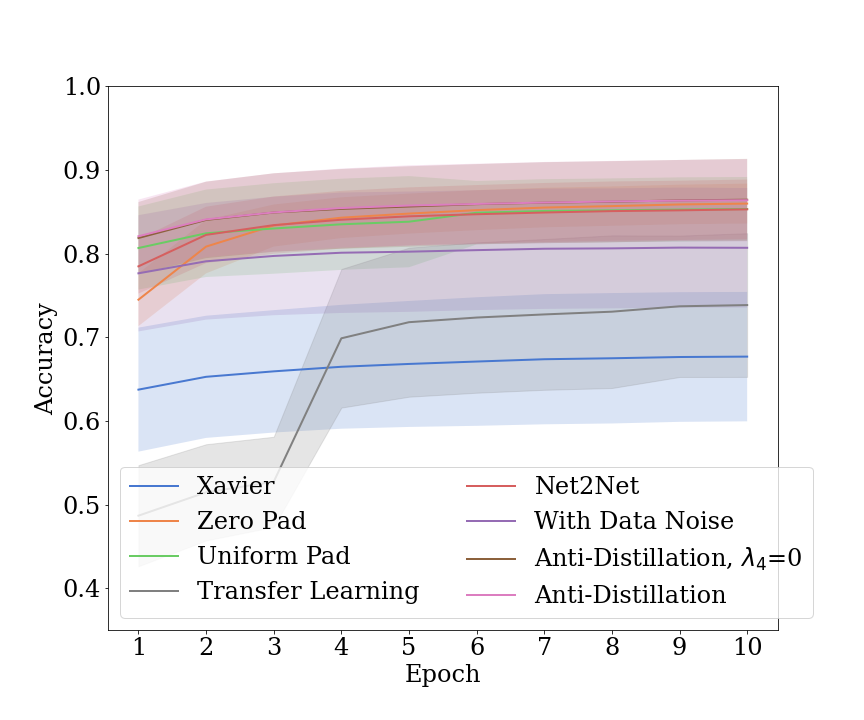
\includegraphics[width=0.5\textwidth]{figures/file.png}
 \caption{Comparison of validation accuracy for different initialization methods}
  \label{fig:1}
\end{figure}
\begin{figure}[!t]
\centering
  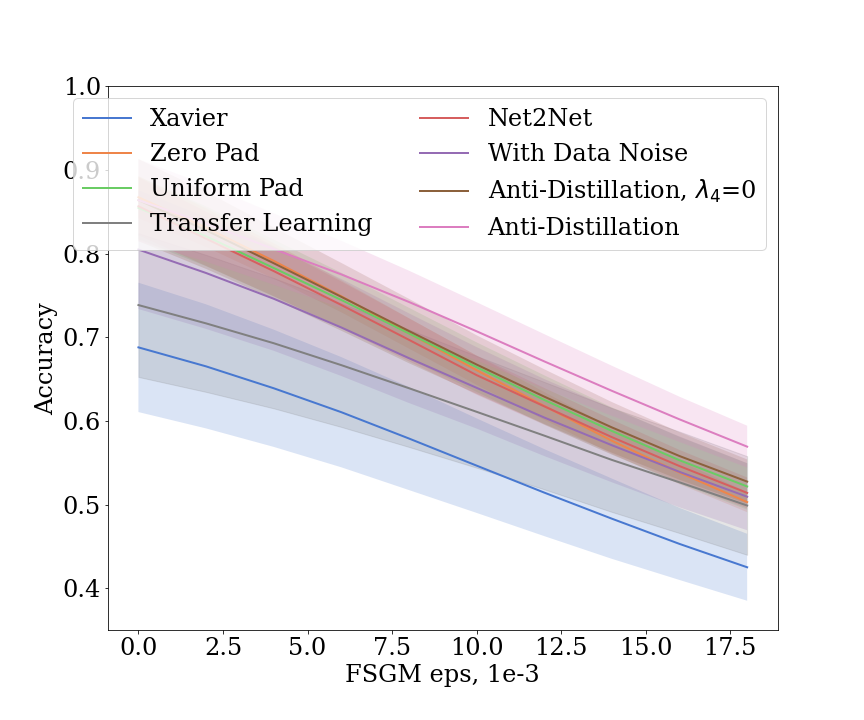
\includegraphics[width=0.5\textwidth]{figures/fsgm.png}
 \caption{Dependence of validation accuracy on adversarial data noise}
  \label{fig:2}
\end{figure}
\begin{figure}[!t]
\centering
  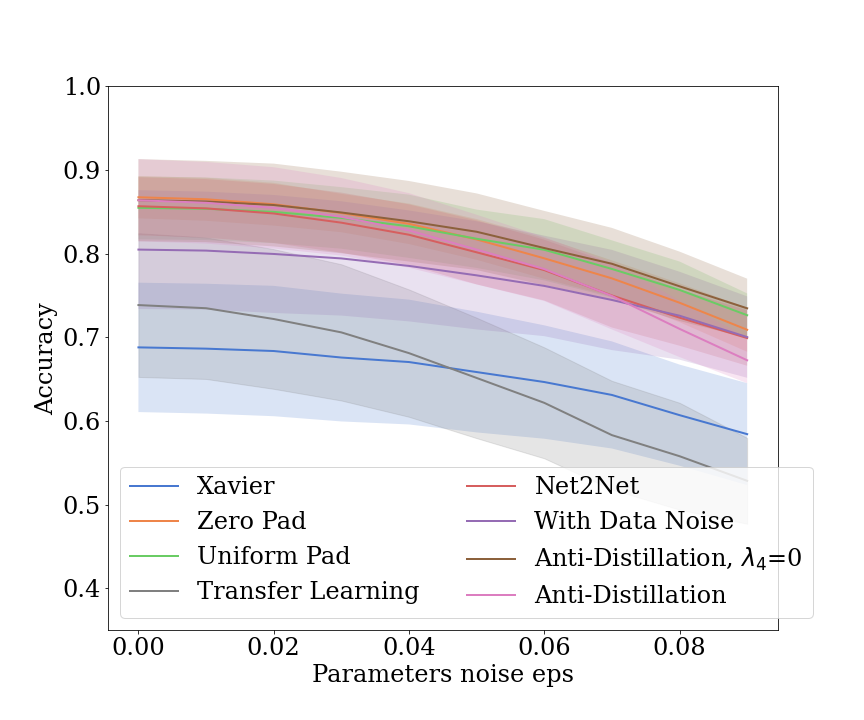
\includegraphics[width=0.5\textwidth]{figures/noise.png}
 \caption{Dependence of validation accuracy on noise intensity parameter $\varepsilon$}
  \label{fig:3}
\end{figure}

\subsection{Error analysis}

The dataset $\mathfrak{D}_2$ set consists of Fasion-MNIST and $\mathfrak{D}_1 = \{(\textbf{x}, y) \;|\; (\textbf{x}, y) \in \mathfrak{D}_2, y \in C_1\}$, $C_1 \subset C_2$, $C_1 = \{0, \dots 4\}, C_2 = \{0, \dots 9\}$. 


As seen in Figure \ref{fig:1} models utilizing Anti-Distillation in average have smaller variance and higher accuracy than models with different initialization of parameters. Training model from scratch turned out to be not the best solution. The proposed method gives us better results with lower number of iterations for convergence. Note, that we did not consider the number of iterations required for the teacher model extension which also requires an optimization procedure. We argue that in many real-life cases this time can be neglected as the proposed method allow us to extend the teacher model once using only the basic dataset $\mathfrak{D}_1$ for further use in multiple student training tasks~\cite{sun2019meta}.

The Figure \ref{fig:2} shows that Anti-Distillation is the most adversarial attack-resistant method of initializing model parameters, since it has the highest validation accuracy with a large margin at high noise levels.

In Figure \ref{fig:3}, we can see that the Anti-Distillation method without Hessian regularization ($\lambda_4=0$) is the most robust to normal noise in the model parameters as it retains the highest accuracy at the maximum considered noise level.

\begin{table}[!h]
\caption{\label{acc_tab} Accuracy on validation set.}

 \begin{tabular}{|c|c|c|c|}
        \hline
        Initialization method & \makecell{Accuracy} &  \makecell{FSGM-attack} & \makecell{
Noise in \\parameters} \\

    \hline
    Xavier & 0.68 $\pm$ 0.08 & 0.42 $\pm$ 0.04 & 0.58 $\pm$ 0.06\\
    \hline
Zero Pad & \textbf{0.86 $\pm$ 0.02} & 0.50 $\pm$ 0.01 & 0.71 $\pm$ 0.03\\
\hline
Uniform Pad & 0.85 $\pm$ 0.04 & 0.52 $\pm$ 0.03 & \textbf{0.73 $\pm$ 0.03}\\
\hline
Transfer Learning & 0.74 $\pm$ 0.09 & 0.50 $\pm$ 0.06 & 0.53 $\pm$ 0.05\\
\hline
Net2Net & 0.85 $\pm$ 0.04 & 0.51 $\pm$ 0.02 & 0.70 $\pm$ 0.03\\
\hline
With Data Noise & 0.81 $\pm$ 0.07 & 0.51 $\pm$ 0.03 & 0.70 $\pm$ 0.05\\
\hline
Anti-Distillation, $\lambda_4$=0 & \textbf{0.86 $\pm$ 0.05} & 0.53 $\pm$ 0.03 & \textbf{0.73 $\pm$ 0.04}\\
\hline
Anti-Distillation & \textbf{0.86 $\pm$ 0.05} & \textbf{0.57 $\pm$ 0.03} & 0.67 $\pm$ 0.03\\
\hline
\end{tabular}

\end{table}

The results are also presented in the tabular form. The Table \ref{acc_tab} contains data on validation accuracy for different initialization methods after the last training epoch, the validation accuracy values at the highest level of image noise by the adversarial attack and information about the accuracy values for the highest noise level in the model parameters.

\section{Conclusion}
The paper considered the problem of the model extension to a new dataset. We considered a case when the new dataset is more complex than the original one. To deal with it we proposed a new method for transfer knowledge from a simple model to a more complex model, which helps to achieve higher accuracy on \textit{more complex} dataset and makes model more persistent to adversarial noise in input data and normal noise in model parameters. To demonstrate the efficiency of the proposed method we conducted an experiment on Fashion-MNIST dataset. 
 As a next step, we plan to consider other datasets, for example CIFAR-10 \cite{cifar10}, and apply a similar approach to other neural network architectures: CNN and RNN, conduct experiments with different default parameters initialization.

\bibliographystyle{IEEEtran}
\bibliography{ieee}

\end{document}
